%-------------------------------------------------------------------------------------------------------
%-------------------------------------------------------------------------------------------------------
% Sec & Label

\section{Simulation Analysis}
\label{sec:simulation}


%-------------------------------------------------------------------------------------------------------
%-------------------------------------------------------------------------------------------------------
% Intro

In this section, Circuit T3 is reproduced with the help of Ngspice.

Ngspice is a simulator for eletronic circuits that can output a variety of results.
This emulator computes the voltages in every node, as well as the potential difference
between two given nodes. Apart from that, the group made use of the command
{\em .options savecurrents} which also enables the output of the currents that pass
through all branches. Moreover, function to help determine de minimum, maximum and average
of the plots were also used.


Firstly, the outcome of the simulation is shown, as well as a brief explanation
on how it was achived. Afterwards, a comparison is done between those values and
the ones attained in Section \ref{sec:analysis}.



%-----------------------------------------------------------------------
%-----------------------------------------------------------------------
% 			     Results - subsec
% ----------------------------------------------------------------------
% ----------------------------------------------------------------------

\subsection{Simulated results}
\label{subsec:sim_res}


% ----------------------------------------------------------------------
% Text


In this laboratory assignament, the Ngspice script made use of the sames values considered for
the Octave script.


\begin{figure}[ht]
	\centering
	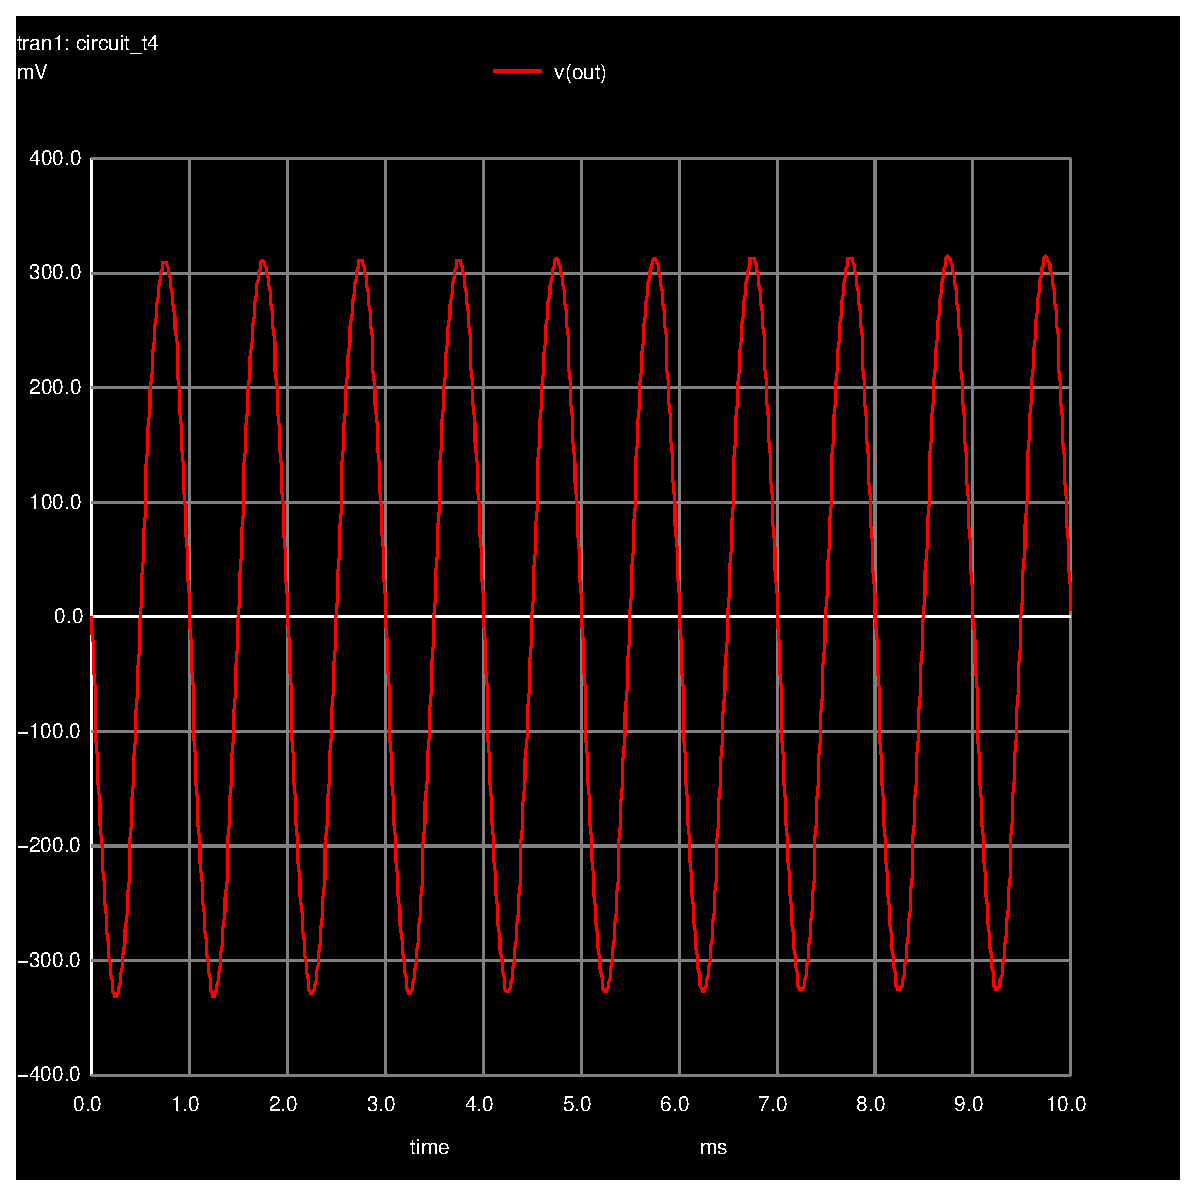
\includegraphics[width=0.5\linewidth]{vo1.eps}
	\caption{Inicial $v_{out}$}
\label{fig:graph_global}
\end{figure}

\begin{figure}[ht]
	\centering
	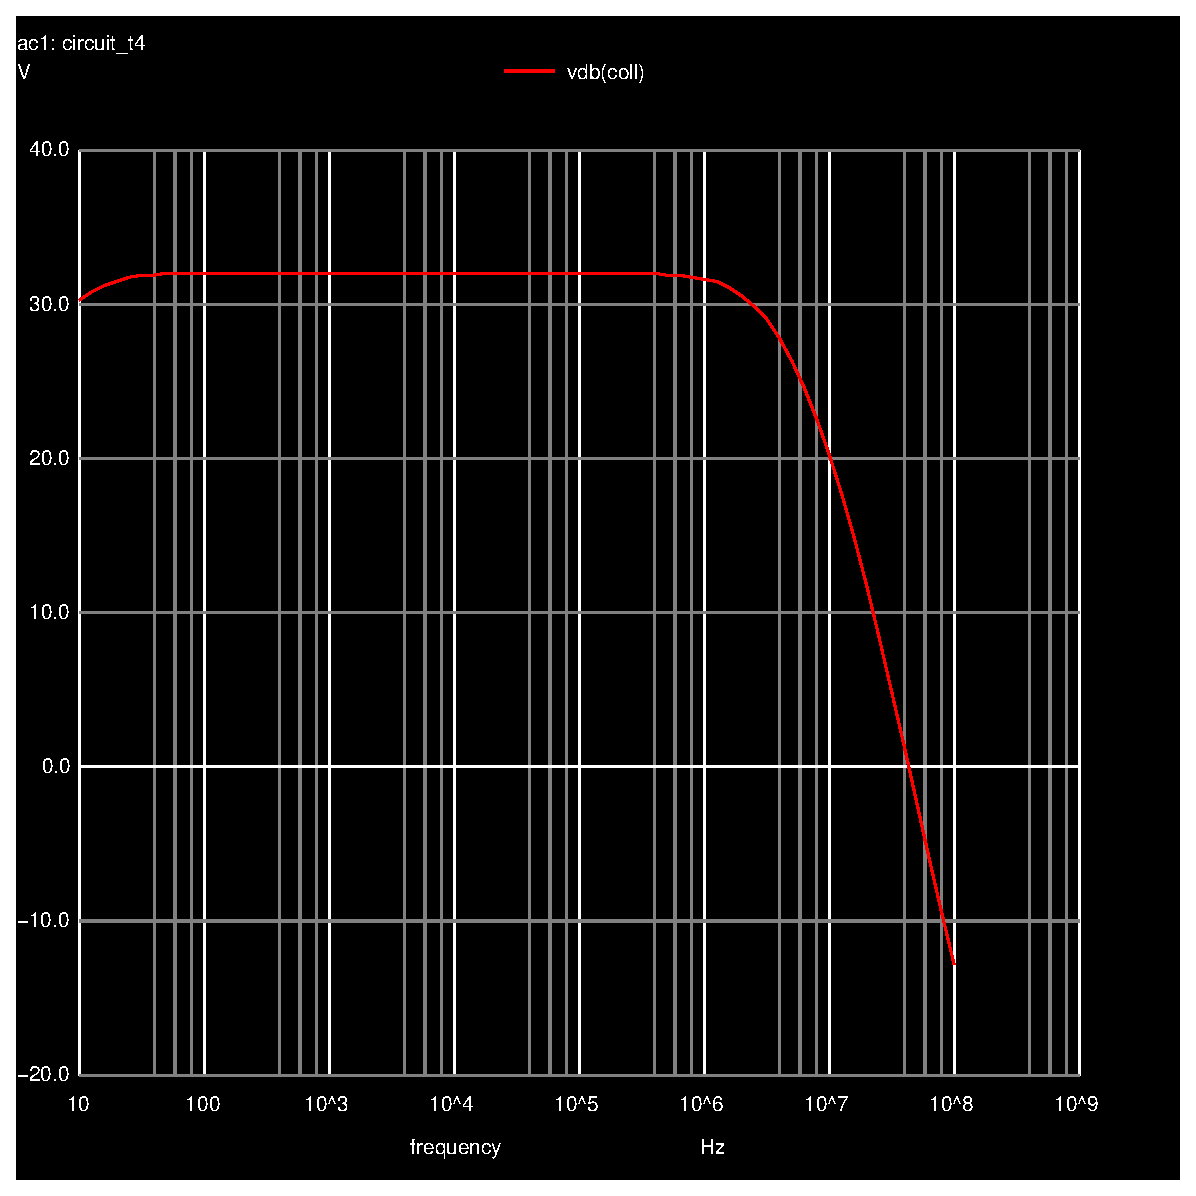
\includegraphics[width=0.6\linewidth]{vo1f.eps}
	\caption{Envelope Detector Circuit $v_{out}$}
\label{fig:EV_vout}
\end{figure}

\begin{figure}[ht]
	\centering
	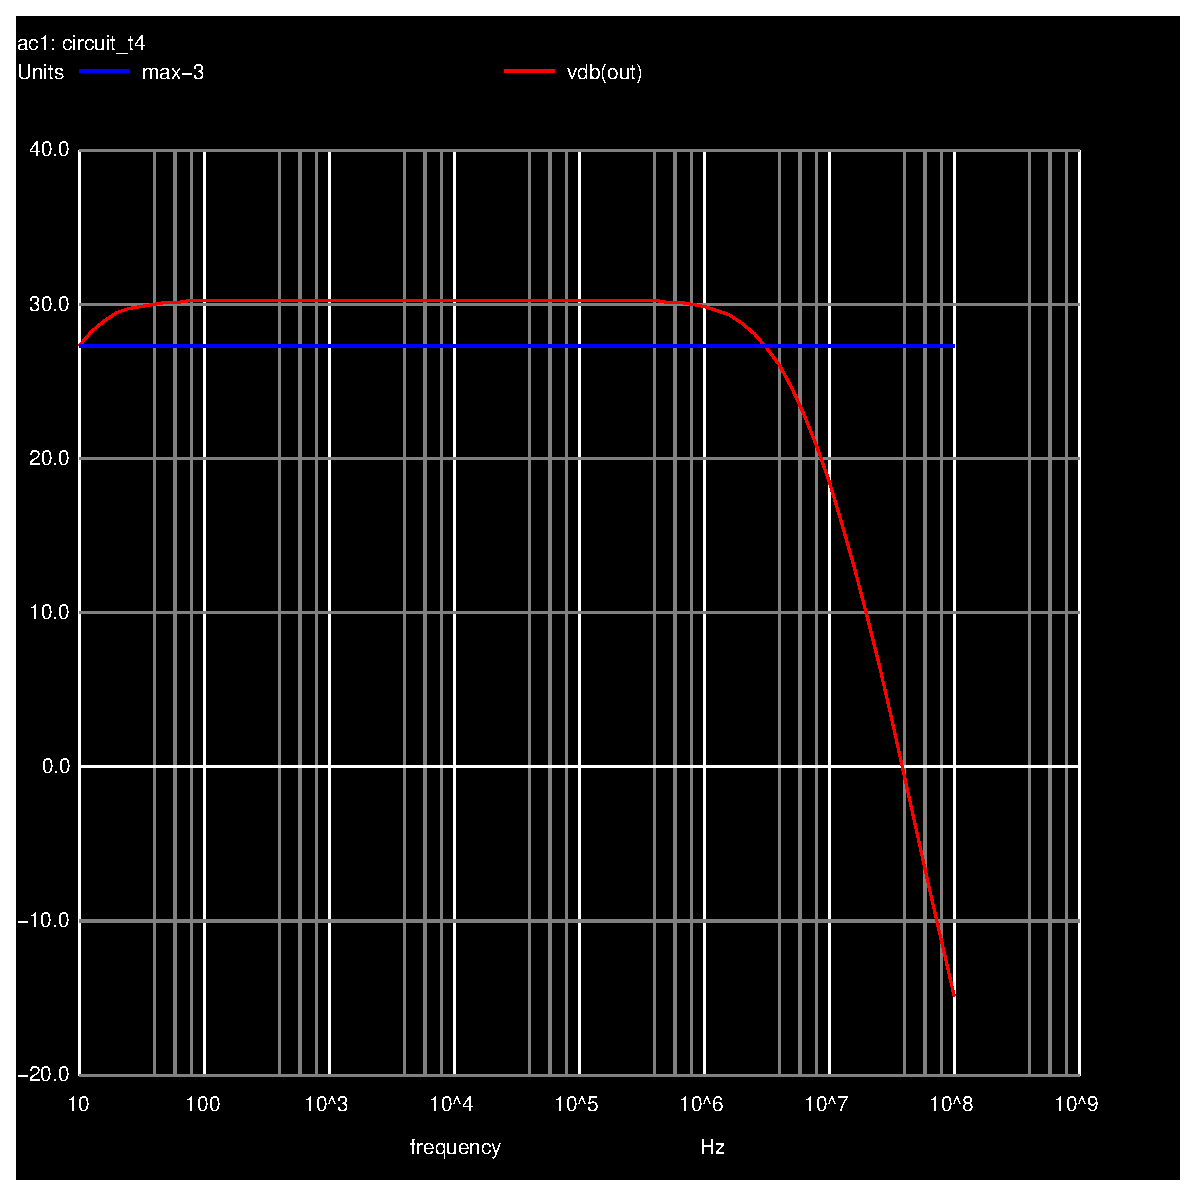
\includegraphics[width=0.6\linewidth]{vo2f.eps}
	\caption{Voltage Regulator Circuit $v_{out}$}
\label{fig:VR_vout}
\end{figure}


As mentioned before, function to determine the minimum, maximum and average of the
plots were also used. Table \ref{tab:trans} shows the average, maximum and minimum
of the plot in Figure \ref{fig:VR_vout}, in that order. In adition, the Ripple
(Vout(MAX) - Vout(MIN)) is also presented.



Lastly, the group also used Ngspice to compute the Merit. This was done, only to confirm
the value obtained in Subsection \ref{subsec:res_the}.


%-----------------------------------------------------------------------
%-----------------------------------------------------------------------
% 			     Comp - subsec
% ----------------------------------------------------------------------
% ----------------------------------------------------------------------

\subsection{Comparison}


% ----------------------------------------------------------------------
% Text




